\section*{Scattered photon energy}
To study the angular dependence of the scattered $\gamma$ a coincidence between the three detectors was selected as trigger of the system. The coincidence between Tagger and Scatterer ensures the detection of the  two collinear 511~keV $\gamma$ from the $^{22}$Na source, then the triple coincidence with the Detector allows to select the Compton scattered $\gamma$ at chosen angle. The data collection was performed over six different angles from 0$^\circ$ to 90$^\circ$, the last one~(90$^\circ$) through a night run because of the lower rate~(see Tab.~\ref{Tab:Rates}). 
\begin{table}[H]
	\centering
	\begin{tabular}{cc}
		\toprule
		\toprule
		 Angle & Rate[Hz] \\
		\midrule
		   0$^\circ$ & 7.3 \\
		20$^\circ$ & 6.8\\
	    40$^\circ$ & 4.6\\
	    60$^\circ$ & 3.4\\
	    70$^\circ$ & 3.1\\
	    90$^\circ$ & 2.3\\
		\bottomrule
		\bottomrule
	\end{tabular}
	\caption{Triple coincidence rates measured in a 30~s time interval.}
	\label{Tab:Rates}
\end{table}

The energy of recoil electrons and scattered $\gamma$ measured by the Scatterer and Detector respectively as a function of scattering angle, is presented in Fig.~\ref{Fig:Scattering_angles}:

\begin{figure}[H]
	\centering
	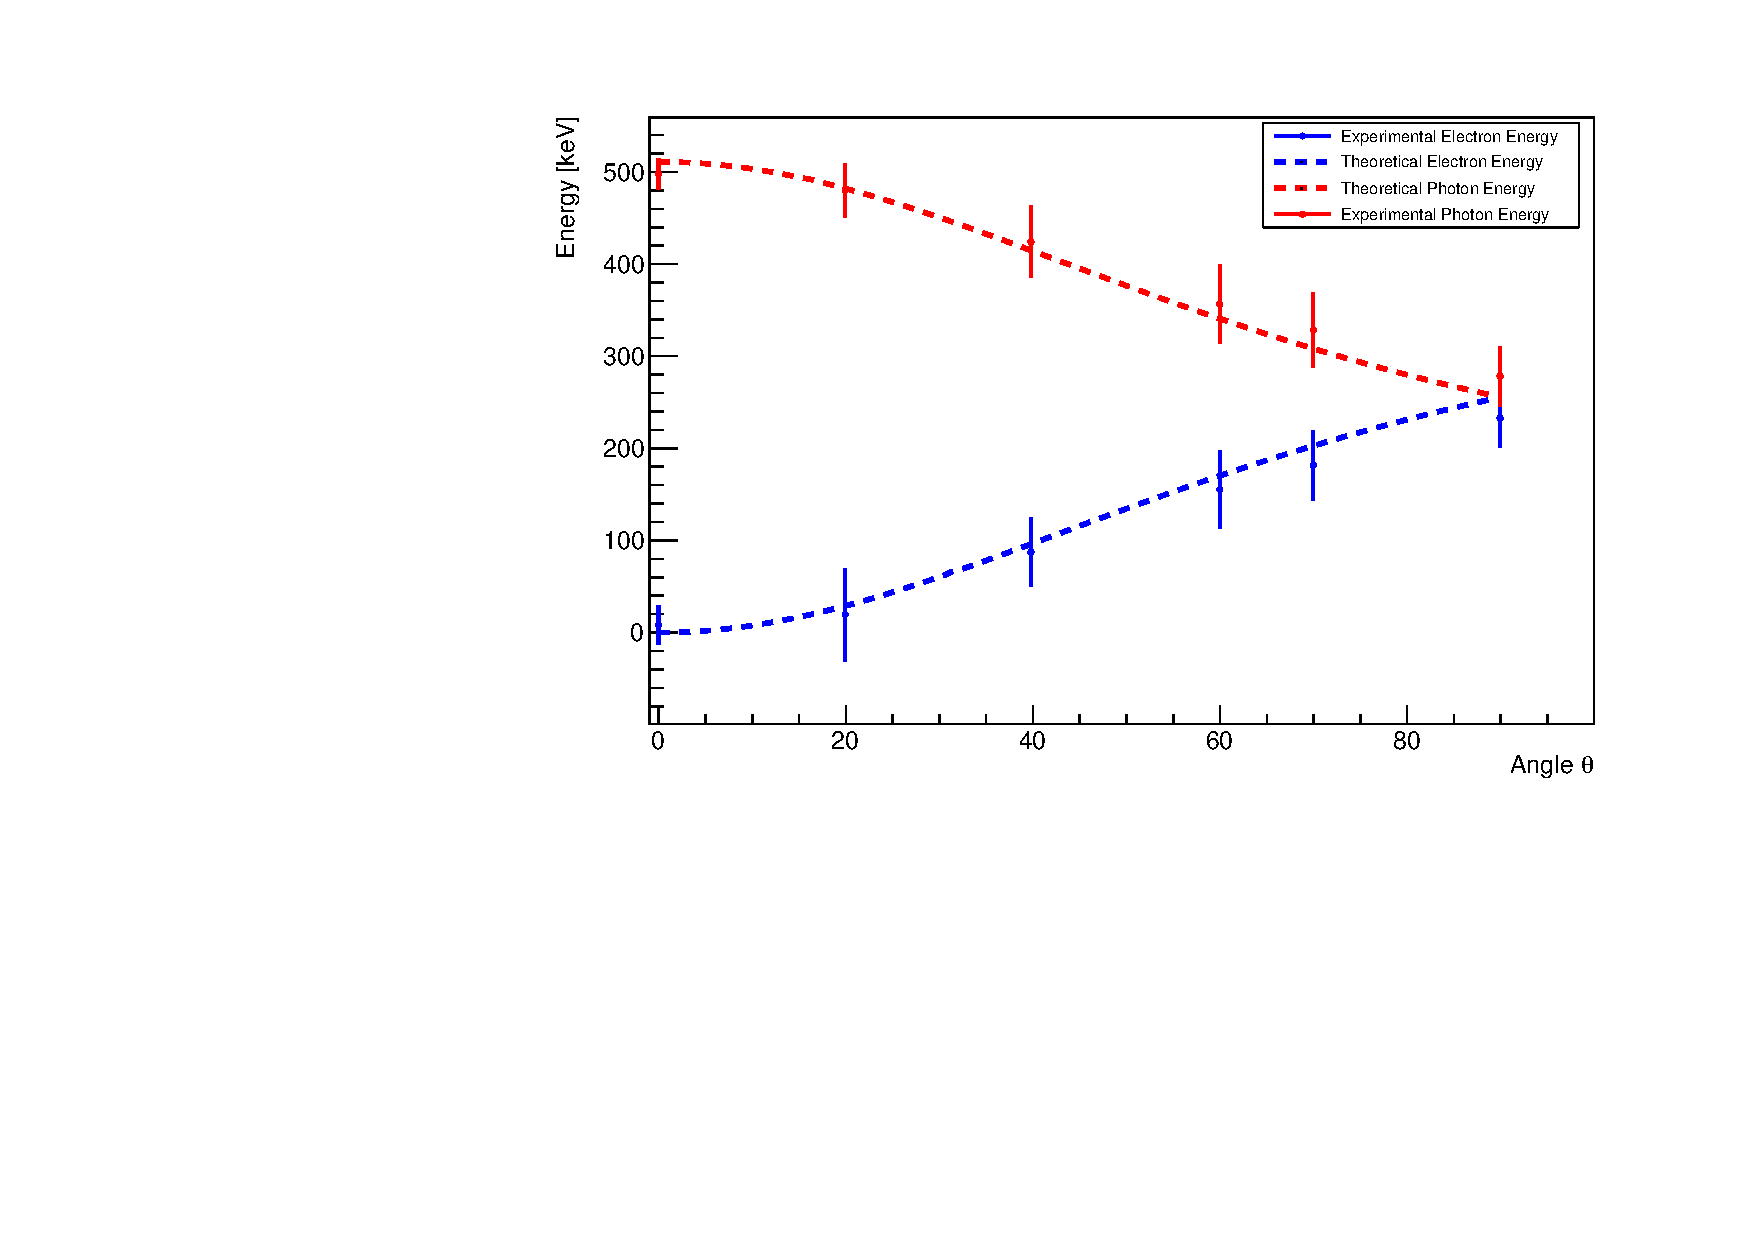
\includegraphics[width=\textwidth]{Angular_photon_energy}
	\caption{Energies of the scattered $\gamma$ and recoil electrons at different scattering angles. The shaped lines represent the theoretical values.}
	\label{Fig:Scattering_angles}
\end{figure}

\newpage
The measured energy values are obtained by a Gaussian fit of the peaks in the acquired spectra of the detectors, and compared to the expected theoretical values predicted by the compton scattering equation:
\begin{equation*}
	h\nu_f=\frac{h\nu_i}{1+\frac{h\nu_i}{m_e c^2}\left(1-cos(\theta)\right)}
\end{equation*}

These measured values are reported in Tab.~\ref{Tab:Scattering_energy} together with the triple coincidences counts for each data acquisition.

\begin{table}[H]
	\centering
	\begin{tabular}{cccc}
		\toprule
		\toprule
		Angle & Count & Recoil Electron energy~[keV] & Scattered Photon energy~[keV] \\
		\midrule
		  0$^\circ$ & 7.3 &   11$\pm$18 &  500$\pm$22\\
		20$^\circ$ & 6.8 &   21$\pm$59 &  486$\pm$28\\
		40$^\circ$ & 4.6 &   78$\pm$39 &  427$\pm$43\\
		60$^\circ$ & 3.4 & 148$\pm$44 &  360$\pm$46\\
		70$^\circ$ & 3.1 & 180$\pm$42 &  327$\pm$44\\
		90$^\circ$ & 2.3 & 231$\pm$33 &  273$\pm$36\\
		\bottomrule
		\bottomrule
	\end{tabular}
	\caption{Recoil electron and scattered $\gamma$ measured energies for six different scattering angles. It is shown also the counts of the triple coincidences which fall in the full energy peak of the Tagger and have a recoil electron energy less than 470~keV~(value selected considering the detector resolution).}
	\label{Tab:Scattering_energy}
\end{table}

Using the 90$^\circ$ spectra~(data set with the highest statistic due to the longer acquisition time) the 2D density plot of Fig.~\ref{Fig:Correlation_Plot} was produced.  A linear fit over the data was performed in order to verify the energy conservation in the Compton scattering process. 
\begin{figure}[h!]
	\centering
	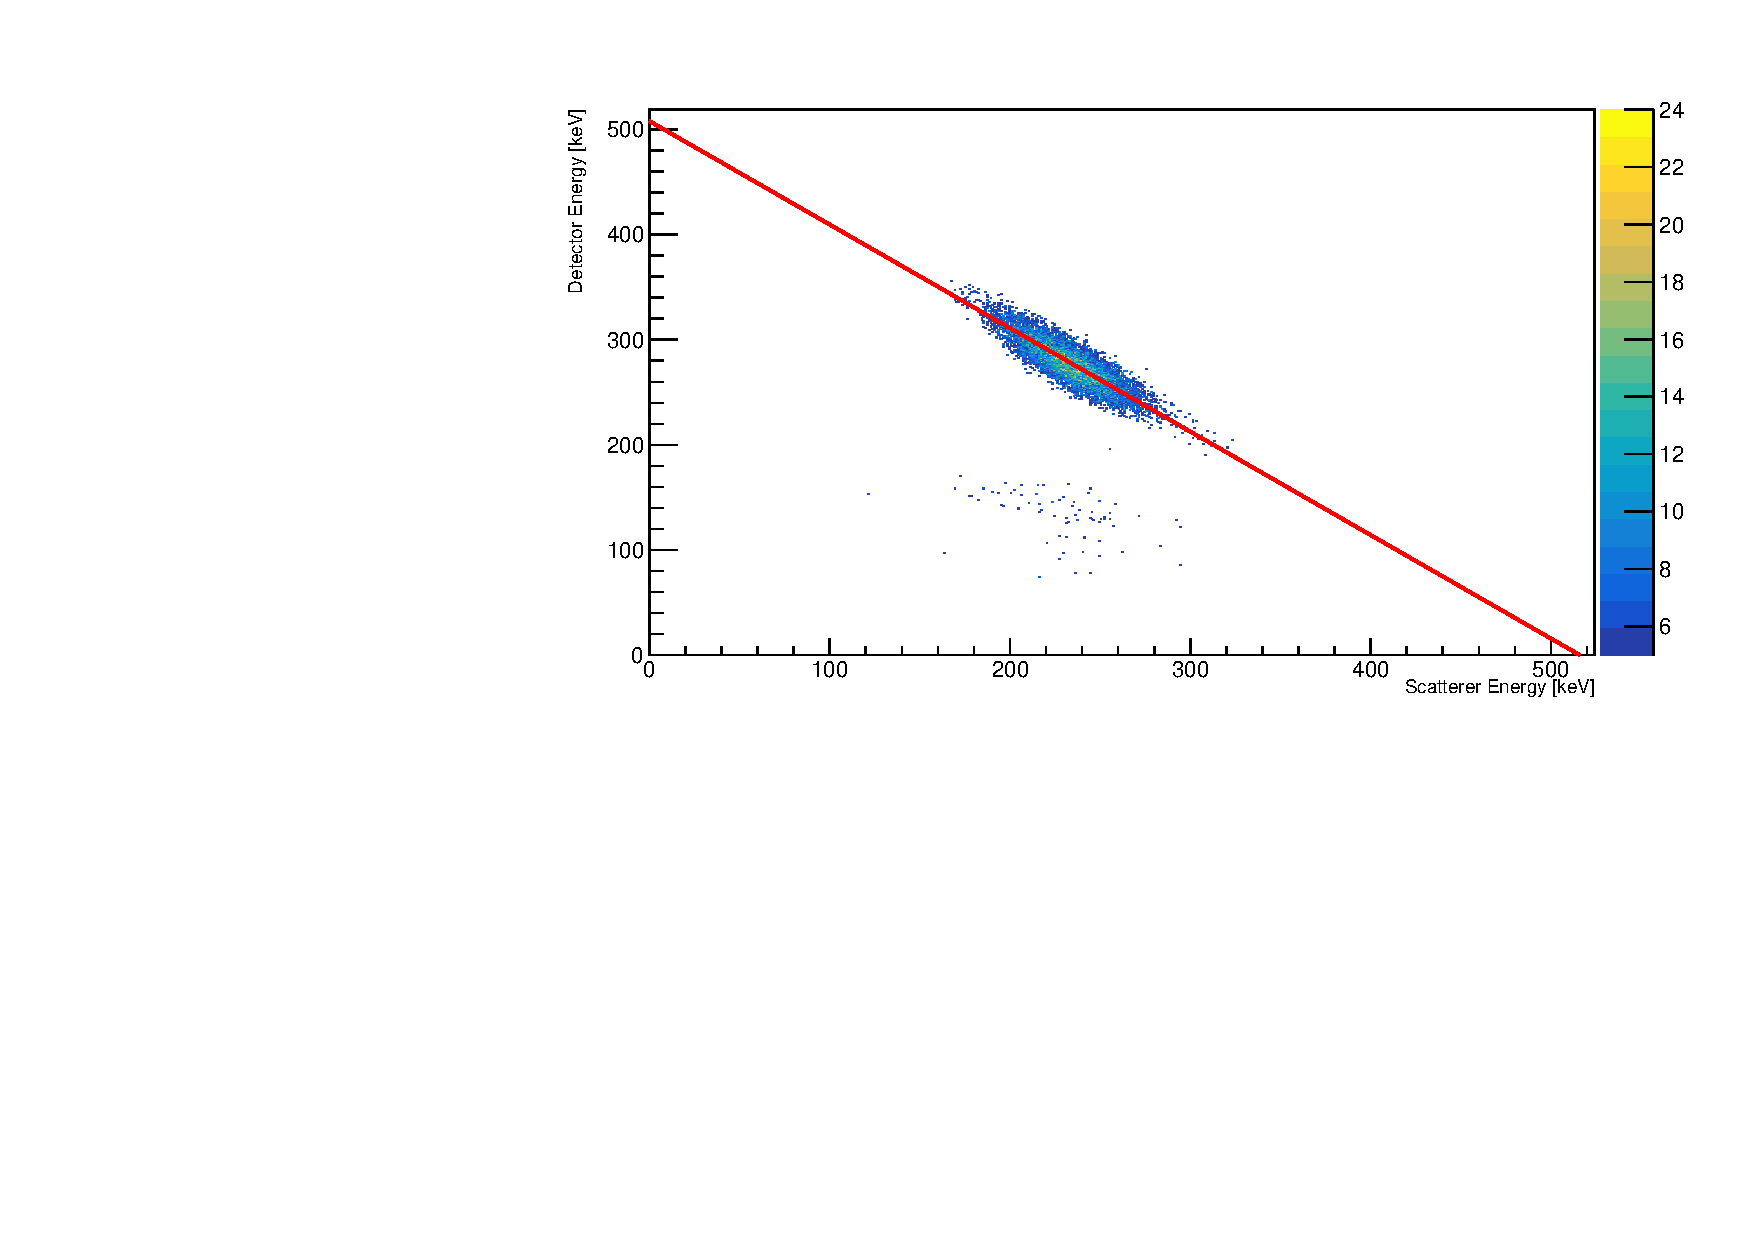
\includegraphics[width=\textwidth]{final_2d_corr_plot}
	\caption{2D density plot of the scattered $\gamma$ energy versus the recoil electron energy. The red fitted line highlight the energy conservation in the scattering process.}
	\label{Fig:Correlation_Plot}
\end{figure}
